\documentclass[border=3pt]{standalone}
% Preâmbulo compartilhado pelos diagramas TikZ da aula 14 (SLAM com EIF)
\usepackage[T1]{fontenc}
\usepackage[utf8]{inputenc}
\usepackage{lmodern}
\usepackage{amsmath}
\usepackage{xcolor}
\usepackage{tikz}
\usetikzlibrary{arrows.meta,angles,quotes,decorations.pathmorphing,decorations.pathreplacing,calc,
                positioning,shapes.geometric,shapes.misc,backgrounds,fit,
                math}

% Paleta (mesma dos SVGs originais)
\definecolor{dblue}{HTML}{2A5B8C}
\definecolor{dorange}{HTML}{B3541E}
\definecolor{dgreen}{HTML}{4A7C59}
\definecolor{dred}{HTML}{9C4B4B}
\definecolor{dcream}{HTML}{F4F1EA}
\definecolor{dshade}{HTML}{DDD7C9}

% Função gaussiana (não normalizada por padrão de escala visual)
\pgfmathdeclarefunction{gauss}{3}{%
  \pgfmathparse{1/(#3*sqrt(2*pi))*exp(-((#1-#2)^2)/(2*#3^2))}%
}

% Estilos comuns (prefixo d... para não colidir com chaves internas do pgf)
\tikzset{
  >={Stealth[length=2mm]},
  dguide/.style={gray!55, dashed, line width=0.4pt},
  daxis/.style={gray!60, line width=0.7pt, ->},
  dbody/.style={fill=black!3, draw=black!80, line width=1pt},
  dacc/.style={draw=dblue, line width=1pt},
  dlbl/.style={black!55, font=\small},
  dsub/.style={black!45, font=\footnotesize},
  dstate/.style={circle, draw=black!80, fill=dcream, line width=1pt,
                 minimum size=17mm, font=\large, inner sep=1pt},
  dobs/.style={circle, draw=black!80, fill=dshade, line width=1pt,
               minimum size=14mm, font=\large, inner sep=1pt},
  dbox/.style={rounded corners=2pt, draw=black!80, fill=dcream, line width=1pt,
               align=center, inner sep=6pt},
  dop/.style={circle, draw=black!80, fill=white, line width=1pt,
              minimum size=6mm, inner sep=0pt, font=\small},
  dtrans/.style={->, dblue, line width=1pt},
  dmeas/.style={->, dorange, line width=1pt},
  dcurve/.style={line width=1pt, dblue},
  dcurveb/.style={line width=1.4pt, dorange},
}

\begin{document}
\hyphenpenalty=10000 \exhyphenpenalty=10000 \tolerance=9999 \emergencystretch=3em
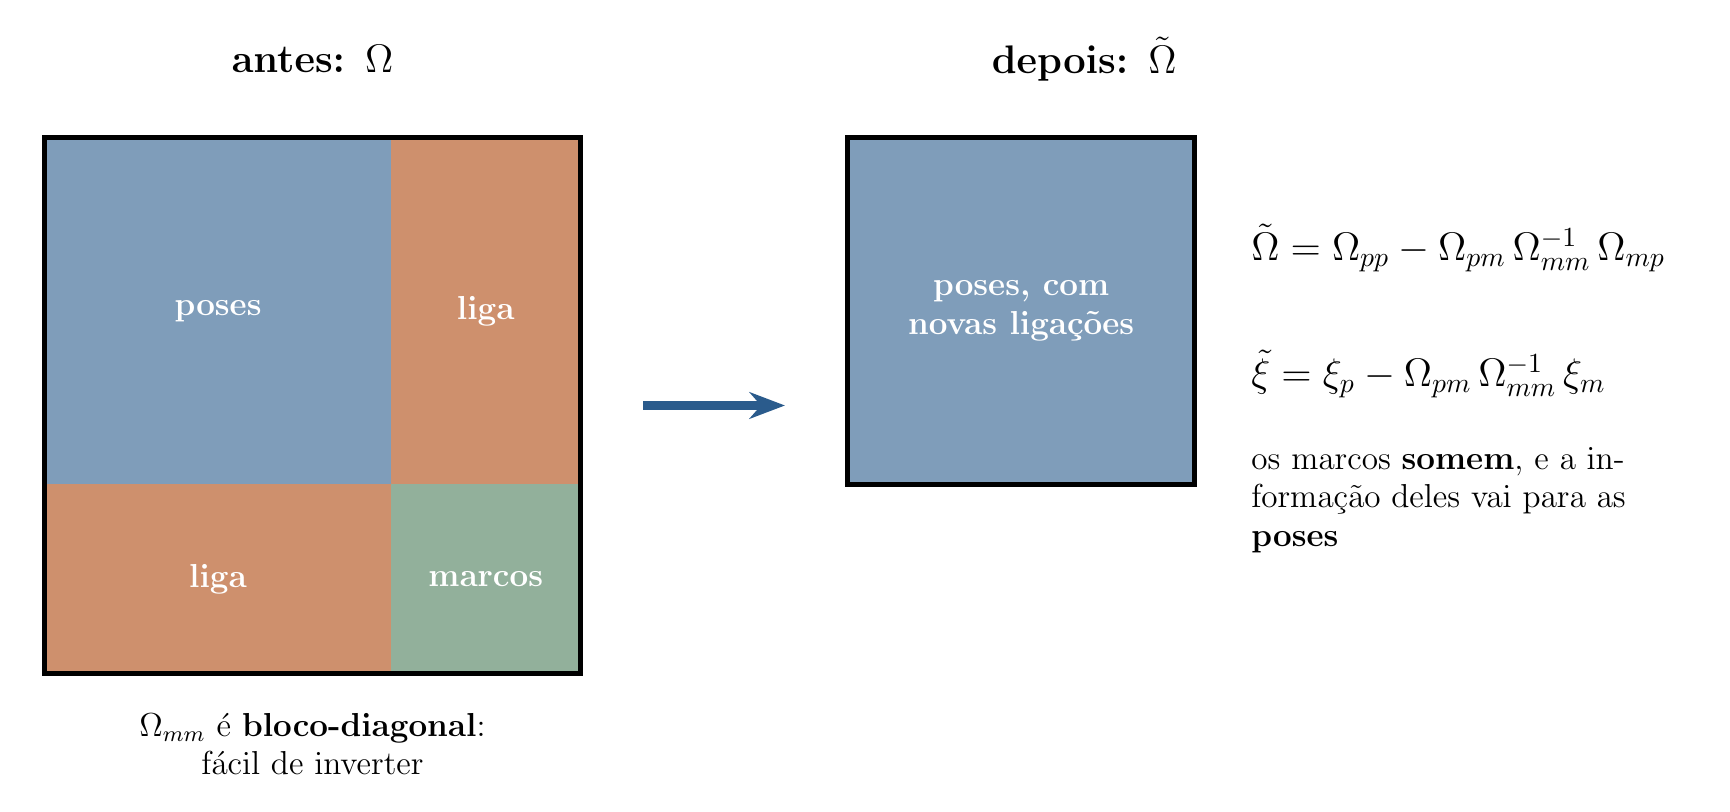
\begin{tikzpicture}[x=1cm,y=1cm]
\def\u{1.0}
\tikzset{bl/.style={draw=black!70, line width=1.4pt}}
\node[font=\Large\bfseries] at (3.4,7.6) {antes: $\Omega$};
\fill[dblue!60] (0,6.6) rectangle (4.4,2.2); \node[font=\large\bfseries, text=white] at (2.2,4.4) {poses};
\fill[dgreen!60] (4.4,2.2) rectangle (6.8,-0.2); \node[font=\large\bfseries, text=white] at (5.6,1.0) {marcos};
\fill[dorange!65] (4.4,6.6) rectangle (6.8,2.2); \node[font=\large\bfseries, text=white] at (5.6,4.4) {liga};
\fill[dorange!65] (0,2.2) rectangle (4.4,-0.2); \node[font=\large\bfseries, text=white] at (2.2,1.0) {liga};
\draw[line width=1.8pt] (0,6.6) rectangle (6.8,-0.2);
\node[font=\large, text width=7cm, align=center] at (3.4,-1.1) {$\Omega_{mm}$ é \textbf{bloco-diagonal}: fácil de inverter};
\draw[dtrans, line width=3pt, -{Stealth[length=4.5mm]}] (7.6,3.2) -- (9.4,3.2);
\node[font=\Large\bfseries] at (13.2,7.6) {depois: $\tilde\Omega$};
\fill[dblue!60] (10.2,6.6) rectangle (14.6,2.2); \node[font=\large\bfseries, text=white, text width=4cm, align=center] at (12.4,4.4) {poses, com novas ligações};
\draw[line width=1.8pt] (10.2,6.6) rectangle (14.6,2.2);
\node[font=\Large, anchor=west] at (15.2,5.2) {$\tilde\Omega=\Omega_{pp}-\Omega_{pm}\,\Omega_{mm}^{-1}\,\Omega_{mp}$};
\node[font=\Large, anchor=west] at (15.2,3.6) {$\tilde\xi=\xi_{p}-\Omega_{pm}\,\Omega_{mm}^{-1}\,\xi_{m}$};
\node[font=\large, anchor=west, text width=5.6cm] at (15.2,2.0) {os marcos \textbf{somem}, e a informação deles vai para as \textbf{poses}};
\end{tikzpicture}
\end{document}
